\section{System Architecture and Design Patterns}
\label{sec:architecture}

\subsection{Architectural Overview}
Software architecture defines the fundamental organization of a system, embodied in its components, their relationships to one another and the environment, and the principles guiding its design and evolution \cite{martin2017clean, pressman2014software}. The Online Auction Management System (BidNexus) employs a \textbf{Multi-Tier Layered Architecture} structured according to the classic Separation of Concerns (SoC) principle.

Figure \ref{fig:arch_layers} conceptually models the flow of control and data dependencies across the four primary tiers.

\begin{figure}[H]
    \centering
    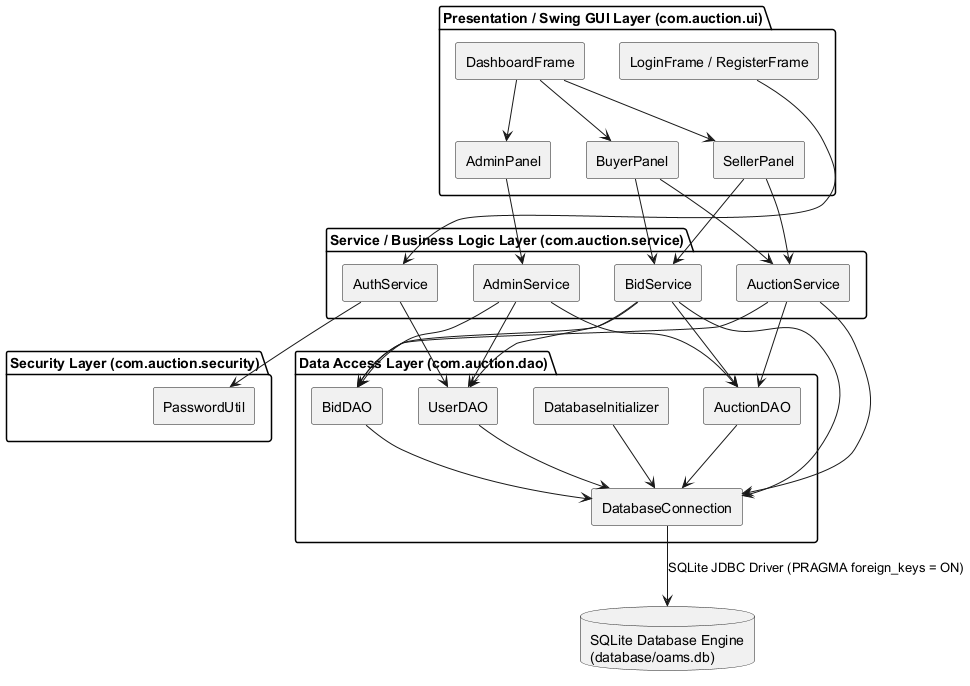
\includegraphics[width=0.88\textwidth]{figures/component_diagram.png}
    \caption{Layered Architectural Organization of BidNexus}
    \label{fig:arch_layers}
\end{figure}

\subsection{Detailed Tier Breakdown}

\subsubsection{1. Presentation Layer (Java Swing GUI)}
The presentation tier encapsulates all user interface rendering, user input capture, and visual feedback. It is housed in the \texttt{com.auction.ui} package. Key components include:
\begin{itemize}
    \item \texttt{LoginFrame} and \texttt{RegisterFrame}: Manage initial credential entry, user role selection, input validation, and delegation to the authentication service.
    \item \texttt{DashboardFrame}: The primary top-level window. Implements role-based dynamic workspace provisioning, rendering customized sidebars and views based on the authenticated user's polymorphic role.
    \item \texttt{BuyerPanel}: Provides auction browsing, keyword search filtering, modal bidding dialogs, and tabular views for ``My Bids'' and ``Auction Results''.
    \item \texttt{SellerPanel}: Provides listing creation dialogs, inventory status monitoring, and itemized bid history tables for seller listings.
    \item \texttt{AdminPanel}: Provides system-wide dashboard metric cards, multi-field user search, auction monitoring, and modal cancellation confirmation dialogs.
    \item \texttt{UiStyle}: A centralized presentation utility that provides consistent color palettes, typography (Segoe UI), card borders, and UI component factories.
\end{itemize}

A critical architectural rule of this layer is that GUI components \textbf{never execute SQL queries or hold direct JDBC references}. All database interactions are delegated through the Service Layer.

\subsubsection{2. Service Layer (Business Logic and Policy Orchestration)}
The service tier, located in \texttt{com.auction.service}, encapsulates business rules, policy constraints, workflow coordination, and transaction management:
\begin{itemize}
    \item \texttt{AuthService}: Orchestrates user onboarding, ensures email uniqueness, invokes password hashing routines, and verifies credentials during login.
    \item \texttt{AuctionService}: Enforces listing policies (e.g., positive reserve prices, future expiration dates), coordinates catalog queries, and conducts lazy expiration sweeps.
    \item \texttt{BidService}: Coordinates competitive bidding, implements row-level locking for concurrency protection, enforces anti-shill policies (blocking sellers from bidding on their own listings), and determines auction winners.
    \item \texttt{AdminService}: Aggregates cross-table platform metrics, coordinates multi-criteria user and auction searches, and validates administrative moderation policies.
\end{itemize}

\subsubsection{3. Security Layer (Cryptographic Utilities)}
The security tier, isolated in \texttt{com.auction.security}, houses \texttt{PasswordUtil}. This utility implements PBKDF2 with HMAC-SHA256, generating unique cryptographically secure 16-byte salts and 256-bit derived hashes with 65,536 iterations. Model objects never store or expose password hashes, adhering to the principle of least privilege.

\subsubsection{4. Data Access Layer (DAO and Persistence)}
The persistence tier, situated in \texttt{com.auction.dao}, encapsulates all SQL query formulation, execution, and Object-Relational mapping:
\begin{itemize}
    \item \texttt{DatabaseConnection}: Manages SQLite JDBC connection lifecycles, ensures the database directory exists, and enforces foreign key support via \texttt{PRAGMA foreign\_keys = ON}.
    \item \texttt{UserDAO}, \texttt{AuctionDAO}, \texttt{BidDAO}: Implement CRUD operations using parameterized \texttt{PreparedStatement} objects. Overloaded methods support both auto-closing standalone connections and caller-managed connections for multi-step transactions.
    \item \texttt{DatabaseInitializer}: Executes schema creation DDL scripts with \texttt{CREATE TABLE IF NOT EXISTS} statements.
\end{itemize}

\subsubsection{5. Relational Database Layer (SQLite)}
The foundational storage engine is SQLite 3, embedded locally at \texttt{database/oams.db}. SQLite provides lightweight, zero-configuration persistence with ACID transactional guarantees.

\subsection{Object-Oriented Design Patterns Applied}
BidNexus applies several classical design patterns to solve common architectural problems:

\paragraph{1. Data Access Object (DAO) Pattern \cite{gamma1994design}:}
The DAO pattern abstracts and encapsulates all access to the database. By providing explicit interfaces (\texttt{UserDAO}, \texttt{AuctionDAO}, \texttt{BidDAO}), the rest of the application remains completely decoupled from SQLite-specific dialect nuances.

\paragraph{2. Model-View-Controller (MVC) Idiom:}
The application adheres to MVC principles within Java Swing:
\begin{itemize}[noitemsep]
    \item \textbf{Model:} Domain entities (\texttt{User}, \texttt{Auction}, \texttt{Bid}) represent application state.
    \item \textbf{View:} Swing panels and frames render data into tables and cards.
    \item \textbf{Controller:} Service classes and action listeners process user input, mutate state, and trigger UI updates.
\end{itemize}

\paragraph{3. Dependency Injection (Constructor Injection):}
Classes receive their dependencies through constructor arguments rather than instantiating them internally. For example, \texttt{BidService} accepts \texttt{DatabaseConnection}, \texttt{AuctionDAO}, \texttt{BidDAO}, and \texttt{UserDAO}. This decouples components and facilitates automated unit testing using temporary in-memory database instances.

\paragraph{4. Immutable Domain Entity Pattern \cite{bloch2018effective}:}
Domain models are constructed as immutable objects with \texttt{private final} fields and no setters. This prevents unintentional mutation and ensures thread-safe data transfer across UI and service layers.

\subsection{Cross-Layer Data Flow}
Figure \ref{fig:data_flow_trace} illustrates how a user action traverses the architectural tiers during a bid submission.

\begin{figure}[H]
    \centering
    \begin{minipage}{0.95\textwidth}
        \centering
        \fbox{
        \parbox{0.9\textwidth}{
        \centering
        \vspace{0.2cm}
        \textbf{Presentation Tier (\texttt{BuyerPanel})}\\[0.1cm]
        Captures bid amount $\rightarrow$ Validates numeric format $\rightarrow$ Calls \texttt{BidService.placeBid()}\\[0.2cm]
        $\boldsymbol{\downarrow}$\\[0.2cm]
        \textbf{Service Tier (\texttt{BidService})}\\[0.1cm]
        Opens JDBC connection $\rightarrow$ Begins Transaction (\texttt{setAutoCommit(false)}) $\rightarrow$\\
        Executes Row Lock $\rightarrow$ Verifies Invariants (Eligibility, Status, Expiration, Amount)\\[0.2cm]
        $\boldsymbol{\downarrow}$\\[0.2cm]
        \textbf{Data Access Tier (\texttt{BidDAO} \& \texttt{AuctionDAO})}\\[0.1cm]
        Executes Parameterized SQL: \texttt{INSERT INTO bids ...} $\rightarrow$ Maps result to \texttt{Bid} entity\\[0.2cm]
        $\boldsymbol{\downarrow}$\\[0.2cm]
        \textbf{Database Engine (SQLite)}\\[0.1cm]
        Validates CHECK and FK constraints $\rightarrow$ Writes to disk/WAL $\rightarrow$ Acknowledges Commit\\[0.2cm]
        $\boldsymbol{\downarrow}$\\[0.2cm]
        \textbf{Return Path: Service commits $\rightarrow$ Returns \texttt{Bid} $\rightarrow$ GUI updates table and displays confirmation}
        \vspace{0.2cm}
        }
        }
        \caption{End-to-End Control and Data Flow Trace for Bid Placement}
        \label{fig:data_flow_trace}
    \end{minipage}
\end{figure}
